
\section{Formative Interviews and Design Goals}

cut out to save space:

\begin{figure}
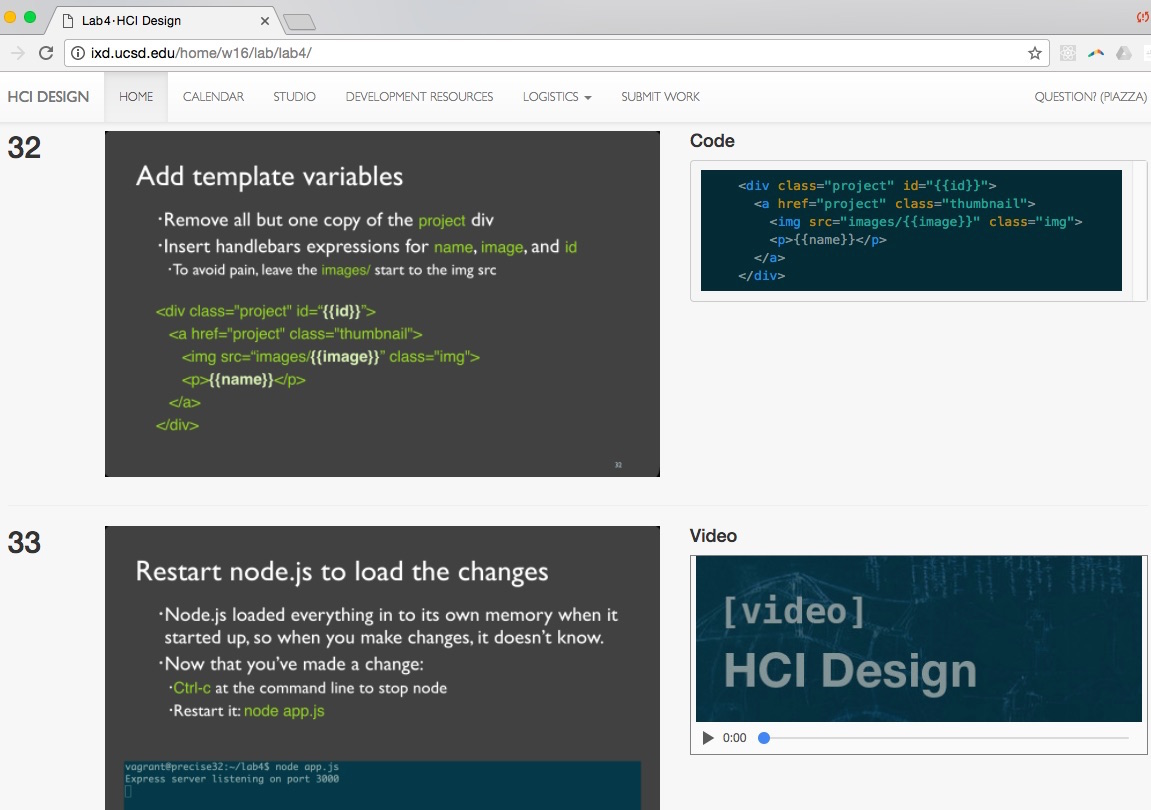
\includegraphics[width=\columnwidth]{figures/torta/ixd-lab-slides.jpg}

\caption{A mixed-media tutorial for web programming that was manually
created for an HCI course~{\protect \cite{ixd}}. Each tutorial is up to
100 steps consisting of PowerPoint slides mixed with code snippets and
videos.}

\vspace{-1em} % stent

\label{fig:ixd-lab-slides}
\end{figure}

To discover the challenges faced by people who manually create
mixed-media software tutorials, we interviewed four teaching
assistants responsible for creating web programming tutorials for an
introductory HCI course~\cite{ixd}.

%Our interviews were semi-structured and focused on walking through their
%process of making, updating, and presenting these tutorials.

In this course, students build full-stack web applications with a mix of
tools such as Git for version control, Node.js for server-side
development, Handlebars for templating, Bootstrap for responsive CSS,
and Heroku for live deployment to the web. Students come into the course
from a diverse variety of majors and widely varying levels of prior programming
experience, so the staff teaches weekly programming tutorials to get
everyone acquainted with the mechanics of web development (e.g., setup,
coding, testing, online deployment). Since these tutorials must
coordinate across multiple command-line and GUI applications, they are
representative of the sorts of tutorials that we would like Torta to
automatically generate.

%Several sets of teaching staff across two universities
%(Stanford and UC San Diego) have iterated on the design of these
%programming tutorials over four years of offering this course and having
%the tutorials used by around 2,000 total students~\cite{ixd}.

Each lesson is a webpage containing a mixed-media tutorial interspersing
PowerPoint slides, video clips, and command/code snippets.
%
Everything is created manually: The staff first makes
a PowerPoint deck (usually around 100 slides) containing step-by-step
instructions, commands to run, code to write/modify, and screenshots
showing expected visual outputs. They export the slides as images to
embed within a webpage and then supplement it with screencast videos and
commands/code that students should copy-and-paste into their terminals.
%
%Students work through the tutorials during class, and the staff walks
%around the classroom to help.
%
From our interviews with teaching assistants, we found three main
bottlenecks in creating these tutorials and deploying them during
in-class lab sessions:

\textbf{\emph{PowerPoint slides versus screencast videos}}: Students
greatly preferred reading the PowerPoint slides since those were easily
skimmable, but the staff found them far more tedious to create since
they needed to first demonstrate their actions and then manually
copy-and-paste all commands, code, expected outputs, and screenshots
into the slides. Also, sometimes the slides did not go into enough
detail or skipped steps due to staff oversight or simply lack of prep time. In contrast, screencast videos were much easier for staff to record and
contain all necessary details, but were harder for students to browse.
The staff struck a compromise by placing slides and videos side by side
on the webpage, using videos to showcase
dynamic events such as GUI interactions and web animations.

\textbf{\emph{Slides, videos, and code are disconnected}}: Besides
slides and videos, the staff also embedded snippets of code and commands
into tutorial webpages. They did this because
students found it hard to copy-and-paste directly from PowerPoint slides
due to syntax-breaking formatting issues (e.g., bad line breaks, smart
quotes, special characters, incomplete code due to lack of space on
slides), and it is impossible to copy from videos. Additionally, the
staff maintained a GitHub repository of skeleton starter code and helper
scripts for students to build upon when following these tutorials. This
heterogeneous setup meant that when the staff created or updated each
tutorial, they had to manually keep four disparate data sources all
updated and in sync:
PowerPoint slides, videos, command/code snippets, and the GitHub
repository of skeleton code; these disconnects led to numerous bugs in
tutorials.

\textbf{\emph{Hard for students to validate progress}}: When working
through tutorials in class, students were anxious about whether they
were following certain steps properly since the PowerPoint slides did
not always specify the expected effects of each step, and videos were
not available for all steps. Many effects were not immediately
visible on-screen, such as the results of running a Heroku configuration
command. Even worse, when a student does not follow a step properly,
everything may still appear to work, but subtle errors silently
propagate and manifest in later steps with unrelated error messages.
These problems arise because students cannot easily check their
progress. The staff ended up dealing with this by writing
\emph{validation scripts} for each tutorial. When a student runs a
validation script, it checks that their filesystem state, environment
variables, and current directory are what the tutorial expects;
otherwise it prints a targeted error message.

%We reflected on the challenges uncovered by our interviews to formulate
These bottlenecks inspired a set of design goals for Torta:

\begin{itemize}\itemsep0pt

\item \textbf{D1}: Creating a tutorial should be as easy as recording a
screencast video, but tutorials should offer advantages of text-based
formats like easy skimming and copy-paste.

\item \textbf{D2}: A tutorial should automatically encapsulate videos,
textual exposition, code examples, and terminal commands together into
one package instead of in disconnected silos.

\item \textbf{D3}: Users should be able to view the tutorial at
varying levels of detail to accommodate their own expertise level.

\item \textbf{D4}: Users should be able to incrementally validate their progress
as they follow each step of the tutorial.

\end{itemize}